\chapter{DATA C100: Regularization}

\section{General Introduction to Regularization}
There are other ways to prevent overfitting, and regularization is one of them. \\
The brief idea of regularization is to restrain the development on size of parameters. \\
For now, let us borrow a view from some two-parameter model under the gradient descent scheme for optimization:
\begin{ln-fig}{Regularization on Graphical Representation, DATA C100}{}
    \begin{center}
        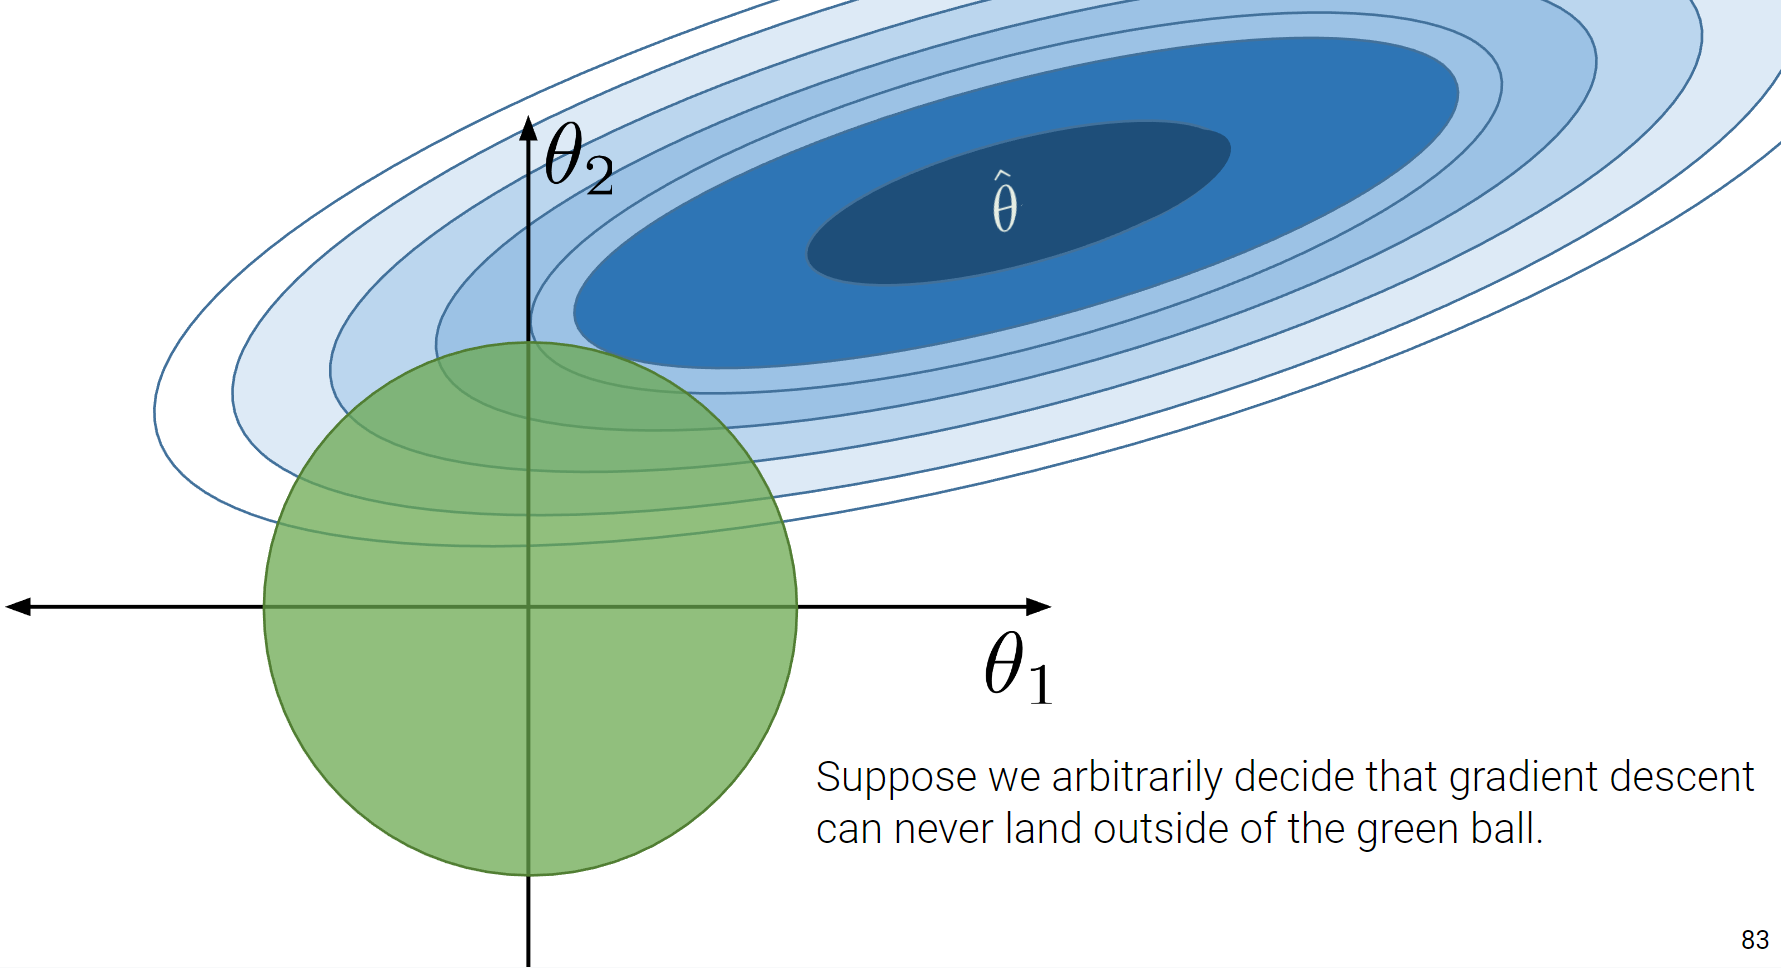
\includegraphics[scale=0.2]{figs/ln07/lin-reg-regularize.png}
    \end{center}
\end{ln-fig}

Now we may ask, how does the radius of this green circle tie in with reducing the complexity of a model. \\
When the green circle is small, we are limited into a less complex model, because the values of each parameters are more restrained. Under the extreme circumstance our green circle is essentially a point, the model would then output $0$ for any possible predictor variable, as the output prediction of model is bound within the green circle. \\
Here, we may also notice that $\theta_0$ is not involved in the model despite being involved in the multiple linear regression line. This would imply that reducing the green circle into a point produces a constant model that merely returns $\theta_0$ as its prediction, which as discussed before, is optimally the mean of every observed value. \\

On the other hand, the larger the green circle's radius is the closer our model behaves to the original model. This allows for more complexity than the previously mentioned constant model. \\
Noticeably then, overly small and overly large radius for the restraining circle each lead to unideal consequences.
\begin{bindenum}
    \item Small radius leads to a constant model with miniscule variance, where validation and training error are both high.
    \item Large radius leads to the original model of regression, which allows for large variance and in exchange brings high validation error with low training error.
\end{bindenum}


However, the nature of variables can lead to their parameters being naturally large. \\
For example, variables that span between $1e-5$ and $1e-3$, perhaps due to unit or measurement, will naturally have larger parameters to help signify their significance in the regression model. \\
To prevent such issues, we should attempt to standardize each data by replacing every data entry with its z-score within its variable category:
\[z_k = \frac{x_k - \mu_k}{\sigma_k}\]
(This is also how the course COMPSCI 70 evaluate each students' performance on an exam, due to its average frequently being around 50\%).

\section{Choices of Regularization}
In other choices of regularization scheme, the circle can be substituted by other shapes.
The green shape on the visual at the beginning of prior section purposes to restrain the parameter size. Below, we will epxlore shapes other than circles that can also fulfill such duty. \\

\subsection{L2 Regularization (Ridge)}
Let us review the visualization of this scheme once again: 
\begin{ln-fig}[sidebyside]{L2 Regularization}{}
    \begin{center}
        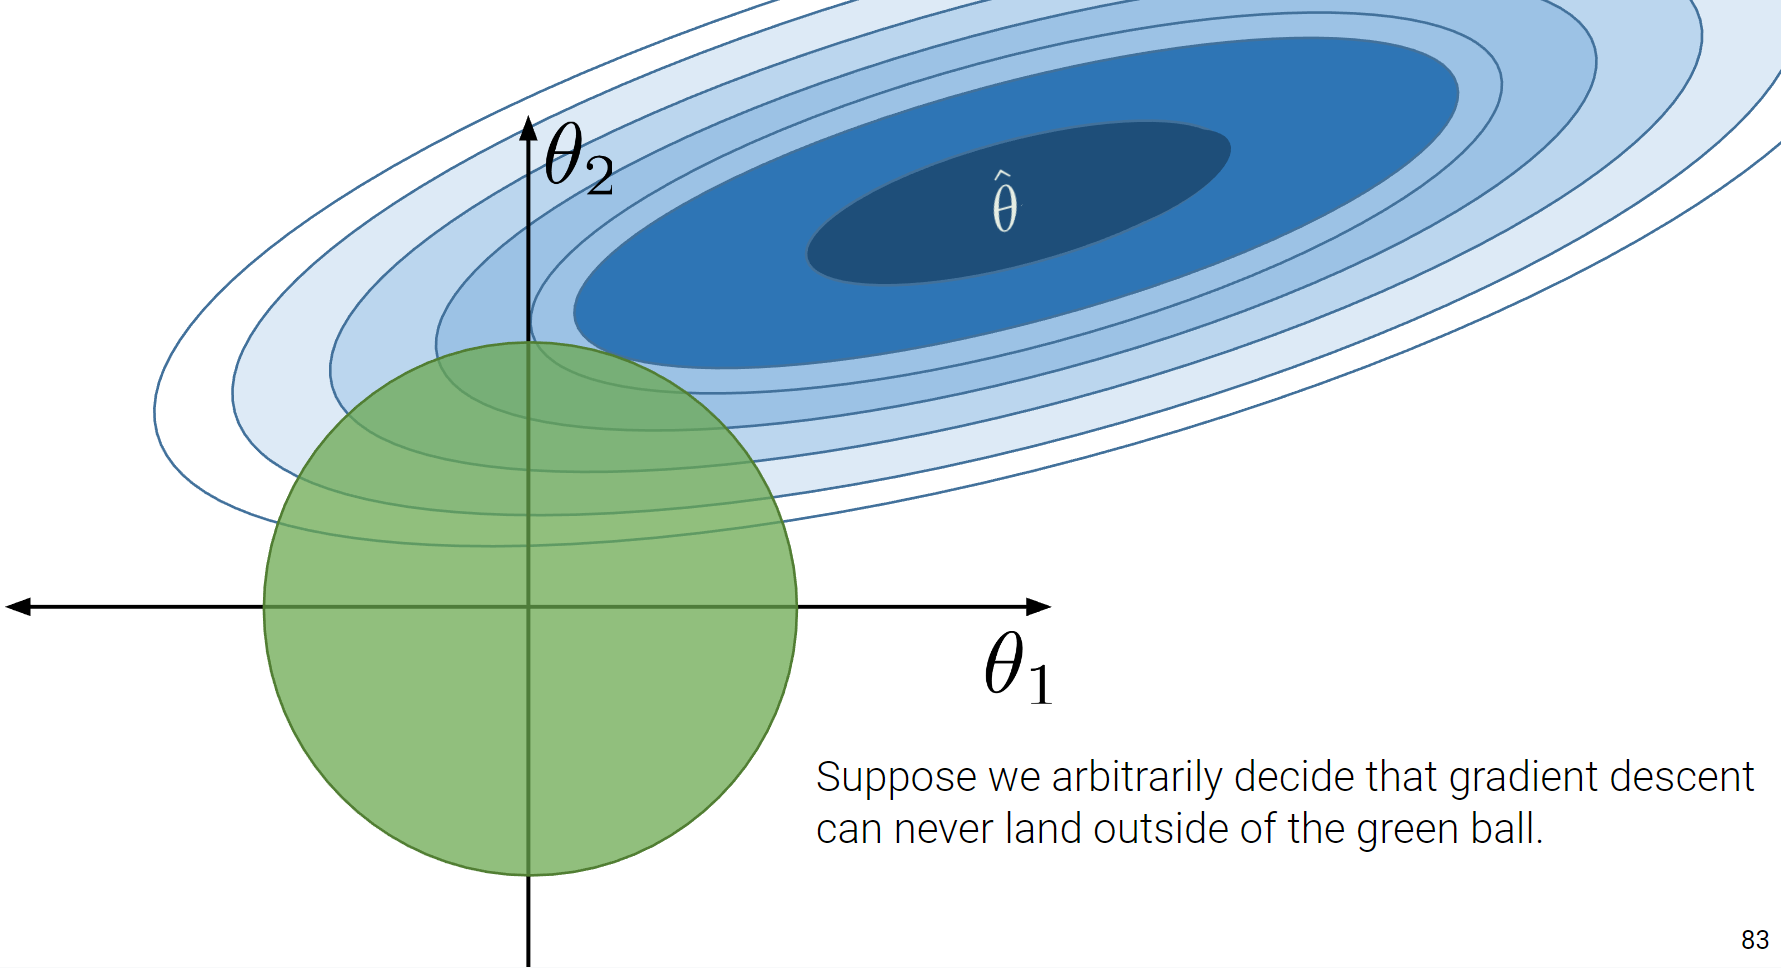
\includegraphics[scale=0.2]{figs/ln07/lin-reg-regularize.png}
    \end{center}
    \tcblower
    L2 Regularization is the scheme where we choose the green shape to be a circle around the origin. In this case, we attempt to minimize the empirical risk, paying attention to this constraint:
    \[\sum_i \theta_i^2 \leq r^2\]
    For an arbitrary, user-chosen $r$ as the radius of the green circle.
\end{ln-fig}

We can run ordinary least squares in the coursework's technology using a ``Ridge'' class as follows:
\setbox\codebox=\hbox{
    \begin{lstlisting}
    >>> from sklearn.linear_model import Ridge
    >>> ridge_model = Ridge(alpha = 10000)
    >>> #alpha is proportional to inverse of radius of
        regularization circle
    >>> ridge_model.fit(design_matrix, y)
    >>> ridge_model.coef_
    an array of optimal model parameters
    \end{lstlisting}
}
\begin{ln-code}{L2 Ridge Regularization in Python}{}
    \usebox\codebox
\end{ln-code}

The reason for which this class is named ``Ridge'' is because the OLS model with an L2 Regularization term is also called \textbf{Ridge Regression} in machine learning:
\begin{ln-define}{Ridge Regression Model}{}
    In a ridge regression model, we find parameters that minimize the following empirical risk as optimal:
    \[R(\theta) = \frac{1}{n}\sum_{i = 1}^n {{(y_i - (\theta_0 + \sum_{j = 1}^d \theta_j \Phi_{i, j}))}^2} + \alpha \sum_{k = 1}^d \theta_k^2\]
    And the multiple of parameter vector's norm at the end of right hand side will offer penalization for parameters whose values are too large. \\
    The optimal solution is, for linear algebra that we will not discuss until EECS 127/189:
    \[\hat{\theta}_{ridge} = {(\X^T \X + n \alpha I)}^{-1} \X^T \Y\]
\end{ln-define}

\subsection{L1 Regularization (LASSO)}
In this scheme, we replace the circle with a cube:
\begin{ln-fig}[sidebyside]{L1 Regularization}{}
    \begin{center}
        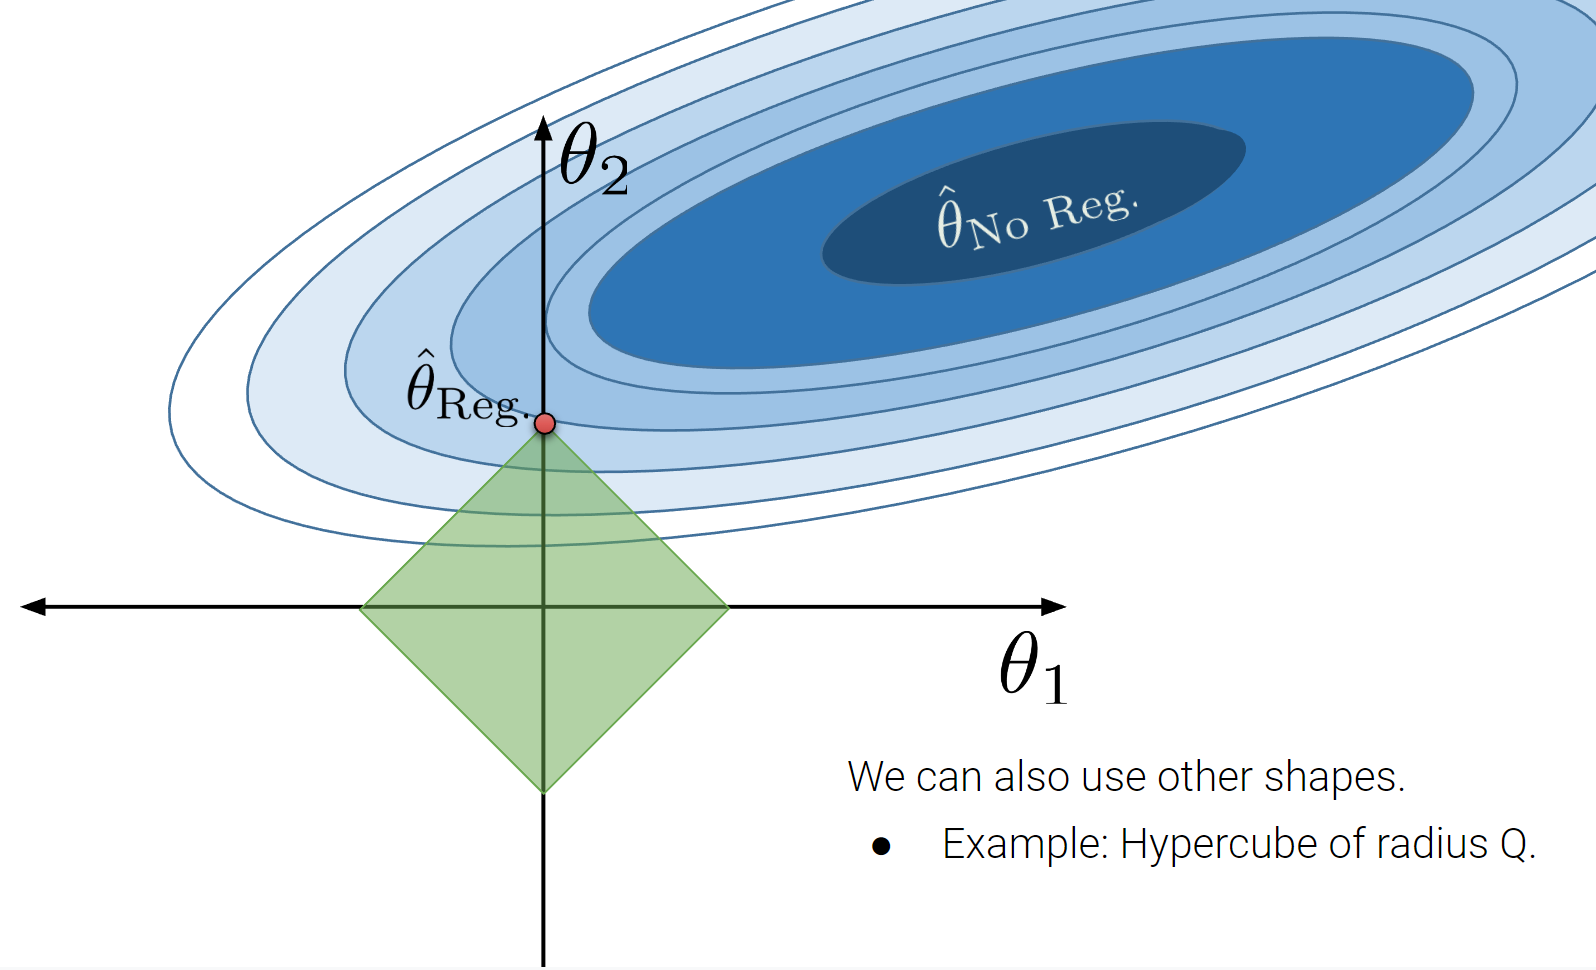
\includegraphics[scale=0.2]{figs/ln07/l1-regularize.png}
    \end{center}
    \tcblower
    Our empirical risk thus becomes:
    \[R(\theta) = \frac{1}{n}\sum_{i = 1}^n {{(y_i - (\theta_0 + \sum_{j = 1}^d \theta_j \Phi_{i, j}))}^2} + \alpha \sum_{k = 1}^d |\theta_k|\]
    Which also involves a penalization term at the end of right hand side.
\end{ln-fig}
In the coursework technology, we may perform L1 regularization on OLS, otherwise known as LASSO Regularization, as noted below:
\setbox\codebox=\hbox{
    \begin{lstlisting}
    >>> from sklearn.linear_model import Lasso
    >>> lasso_model = Lasso(alpha = 10)
    >>> lasso_model.fit(design_matrix, y)
    >>> lasso_model.coef_
    an array of optimal model parameters
    \end{lstlisting}
}
\begin{ln-code}{L1 LASSO Regularization in Python}{}
    \usebox\codebox
\end{ln-code}
\textbf{LASSO Regularization}, or ``Least Absolute Shrinkage and Selection Operator'', tend to involve many zeros in its optimal parameters. In other words, it only chooses a subset of features to use in its regression model. \\

\subsection{Summary of Regularization Choices}
\begin{center}
    \begin{tabular}{c|ccc|c|c}
        Name & Model & Loss & Reg. & Empirical Risk & Solution \\
        \hline
        OLS & $\hat{\Y} = \X \theta$ & L2 & None & $\frac{1}{n}{||\Y - \X \theta||}_2^2$ & $\hat{\theta}_{OLS} = {(\X^T \X)}^{-1} \X^T \Y$ \\
        Ridge & $\hat{\Y} = \X \theta$ & L2 & L2 & $\frac{1}{n}{||\Y - \X \theta||}_2^2 + \lambda \sum_{j = 1}^d \theta_j^2$ & $\hat{\theta}_{OLS} = {(\X^T \X + n\lambda I)}^{-1} \X^T \Y$ \\
        LASSO & $\hat{\Y} = \X \theta$ & L2 & L1 & $\frac{1}{n}{||\Y - \X \theta||}_2^2 + \lambda \sum_{j = 1}^d |\theta_j|$ & no closed form
    \end{tabular}
\end{center}
While it destines the regularized models will have a higher empirical risk than OLS in general, regularization will effectively inhibit overfitting and offer a better in-real-life performance for our model, which is much better than only having a good performance on the training set.
